\documentclass[11pt,a4paper]{article}
\usepackage[margin=21mm]{geometry}
\usepackage[T1]{fontenc}
\usepackage{lmodern}
\usepackage{microtype}
\usepackage{booktabs}
\usepackage{graphicx}
\usepackage{hyperref}
\usepackage{xcolor}
\usepackage{placeins}
\usepackage{enumitem}
\hypersetup{
  colorlinks=true,
  linkcolor=blue,
  urlcolor=blue,
  pdftitle={Passive DS-TWR Deadline Pipeline and Rolling Solver Field Validation}
}
\graphicspath{{figures/}}

\title{Passive DS-TWR Deadline Pipeline\\and Rolling Solver Field Validation}
\author{UWB Module ESP-IDF field test}
\date{28 July 2026}

\begin{document}
\maketitle

\begin{abstract}
This report validates the non-blocking DW3000 deadline pipeline and the
low-latency rolling position solver added to the custom receive-only Passive
DS-TWR protocol. In a static surveyed geometry, deadline scheduling increased
independent position throughput from approximately 63 to 84 updates/s without
an observed accuracy regression. Rolling solving preserved the independent
frame rate while increasing total display updates to 169/s. The deadline
pipeline also reduced combined RESP/FINAL timeout counts by approximately
73\% and removed the large anchor-range bursts present in the legacy
millisecond/blocking scheduler during this test.
\end{abstract}

\section{Objective}

The previous Passive DS-TWR speed-limit study identified the radio transaction
and millisecond receive-loop scheduling path as the principal bottleneck. It
recommended four changes:
\begin{enumerate}[itemsep=2pt,topsep=3pt]
\item instrument POLL TX, delayed RESP TX, FINAL TX/RX, CIA readout, and RX
re-arm;
\item replace millisecond receive-loop scheduling with DW3000 delayed-TX and
deadline-driven state transitions;
\item retain Robust Rotating at 1.0/1.0 ms as the accuracy control;
\item evaluate rolling solves as a distinct low-latency display mode while
reporting independent frames/s separately.
\end{enumerate}

Firmware \texttt{7226cca} implements those changes. The purpose of this field
test is to determine whether they improve speed without sacrificing static
accuracy or destabilising the radio schedule.

\section{Experimental method}

Five modules were flashed once in one simultaneous OTA operation. Four anchors
formed the known \(3\,\mathrm{m}\times3\,\mathrm{m}\) reference square:
A2 \(=(0,0)\), A3 \(=(0,3)\), A4 \(=(3,0)\), and A5 \(=(3,3)\) m. Tag 1
was stationary at the surveyed centre, \((1.5,1.5)\) m. Dynamic anchor
self-localisation remained active, matching the intended operational system
rather than forcing fixed dashboard coordinates.

Every test used Robust Rotating with 1.0 ms RESP and 1.0 ms FINAL timing.
Four 60 s blocks, each preceded by a 10 s warm-up, formed an A--B--C--A
sequence:
\begin{description}
\item[A1] Legacy receive loop, one solve per complete frame;
\item[B] deadline pipeline, one solve per complete frame;
\item[C] deadline pipeline, rolling solves capped at 100 Hz;
\item[A2] return to the Legacy control.
\end{description}

Positions were captured from the dashboard's lossless event stream. Raw solver
and constant-velocity EKF outputs were retained separately. Accuracy for the
rolling block is calculated only from its complete independent-frame
solutions; correlated intermediate rolling results are not counted as
additional independent accuracy samples.

\section{Throughput}

\begin{table}[htbp]
\centering
\small
\begin{tabular}{lrrrr}
\toprule
Mode & independent & rolling & total solver & independent\\
 & frames/s & updates/s & updates/s & samples\\
\midrule
Legacy + Frame A1 & 62.54 & -- & 62.54 & 3,753\\
Deadline + Frame & 84.12 & -- & 84.12 & 5,053\\
Deadline + Rolling & 84.38 & 84.76 & 169.14 & 5,066\\
Legacy + Frame A2 & 63.24 & -- & 63.24 & 3,799\\
\bottomrule
\end{tabular}
\caption{Measured position throughput over each 60 s capture.}
\end{table}

\begin{figure}[htbp]
\centering
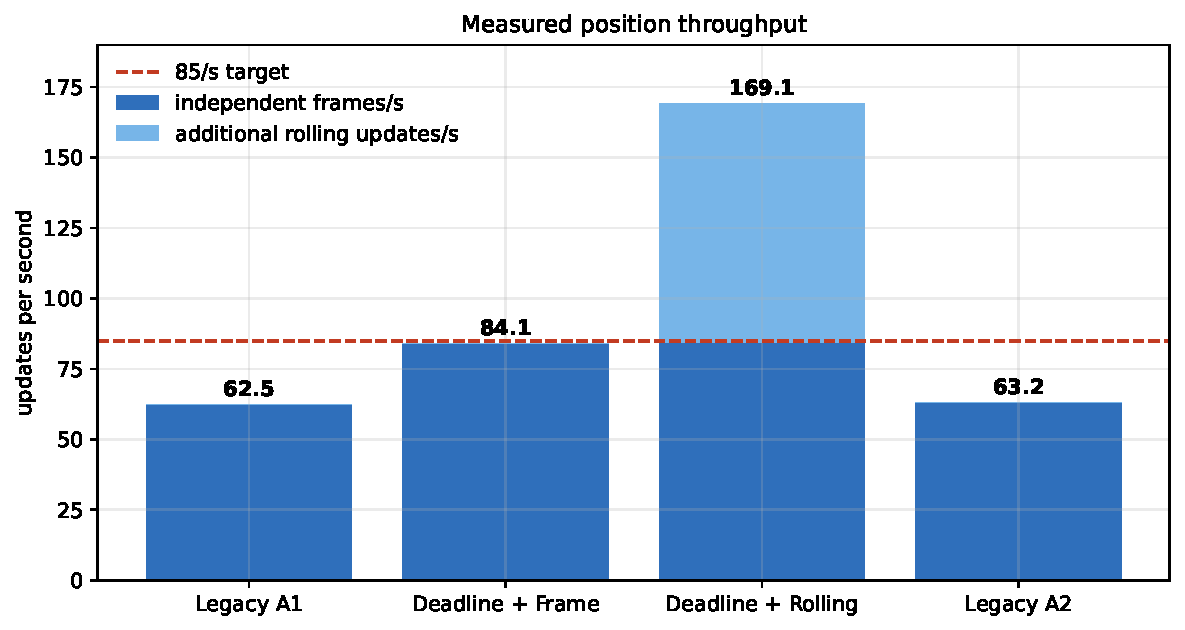
\includegraphics[width=0.92\linewidth]{pipeline_update_rate.pdf}
\caption{Independent frame rate and additional correlated rolling updates.
The rolling solver approximately doubles display refresh while leaving radio
frame throughput unchanged.}
\end{figure}

Deadline scheduling increased independent frame throughput by 34.5\% over A1.
The A2 return control reproduced the Legacy rate, which supports attributing
the gain to the new scheduling pipeline rather than a transient change in
network or dashboard performance. Enabling the rolling solver changed the
independent rate from 84.12 to 84.38 frames/s; consequently, there is no
measured evidence that the added solver work slows the ranging path.

\FloatBarrier
\section{Static position accuracy}

\begin{table}[htbp]
\centering
\small
\begin{tabular}{lrrrrrr}
\toprule
Mode & \multicolumn{2}{c}{EKF error [cm]} &
\multicolumn{2}{c}{raw error [cm]} &
\multicolumn{2}{c}{EKF bias [cm]}\\
\cmidrule(lr){2-3}\cmidrule(lr){4-5}\cmidrule(lr){6-7}
 & RMSE & P95 & RMSE & P95 & \(x\) & \(y\)\\
\midrule
Legacy + Frame A1 & 3.59 & 5.51 & 3.87 & 6.17 & +0.30 & -3.12\\
Deadline + Frame & 3.23 & 5.09 & 3.59 & 5.92 & +1.04 & -2.47\\
Deadline + Rolling & 3.01 & 4.72 & 3.28 & 5.32 & -0.05 & -2.43\\
Legacy + Frame A2 & 5.12 & 7.29 & 5.35 & 8.04 & +1.62 & -4.50\\
\bottomrule
\end{tabular}
\caption{Position errors relative to the surveyed centre. Deadline + Rolling
uses only independent-frame solutions in this accuracy table.}
\end{table}

\begin{figure}[htbp]
\centering
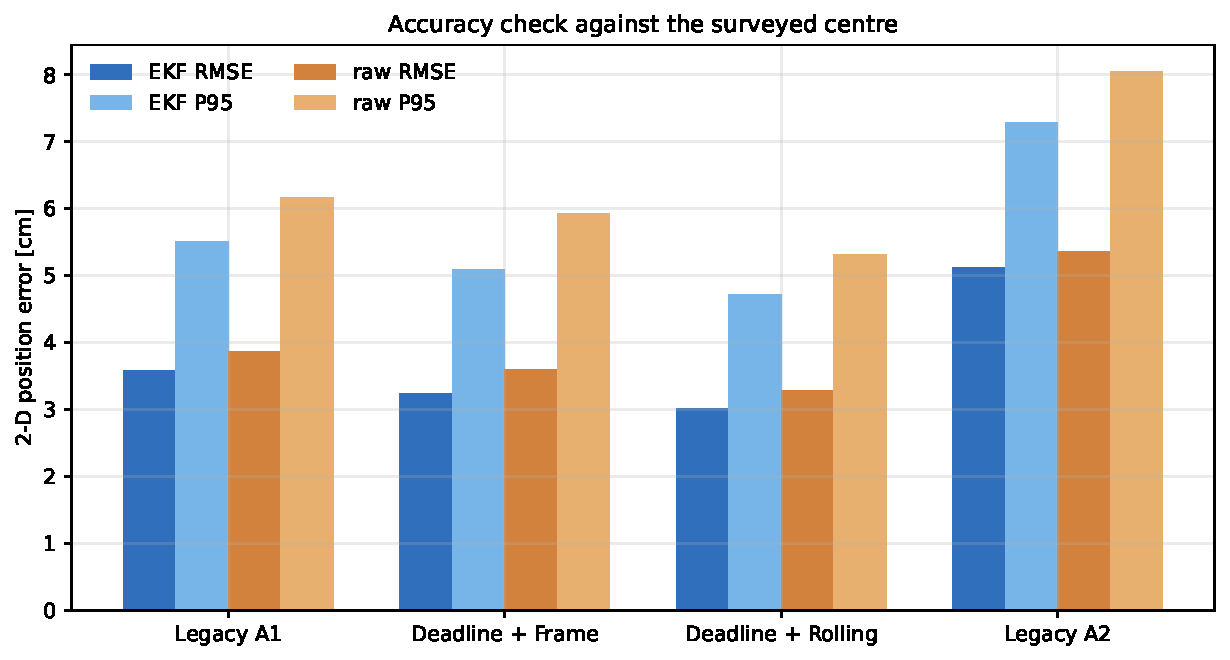
\includegraphics[width=0.94\linewidth]{pipeline_accuracy.pdf}
\caption{Filtered and raw accuracy. The raw results confirm that the accepted
deadline result is not solely an EKF artefact.}
\end{figure}

\begin{figure}[htbp]
\centering
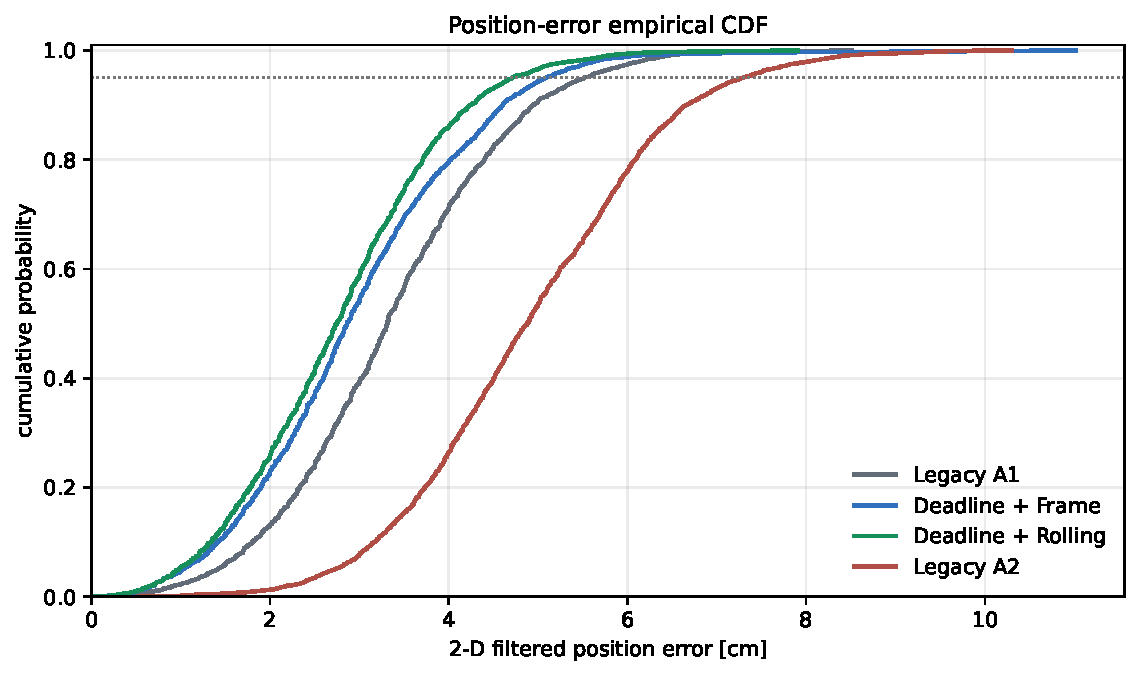
\includegraphics[width=0.88\linewidth]{pipeline_error_cdf.pdf}
\caption{Empirical CDF of filtered 2-D position error.}
\end{figure}

\begin{figure}[htbp]
\centering
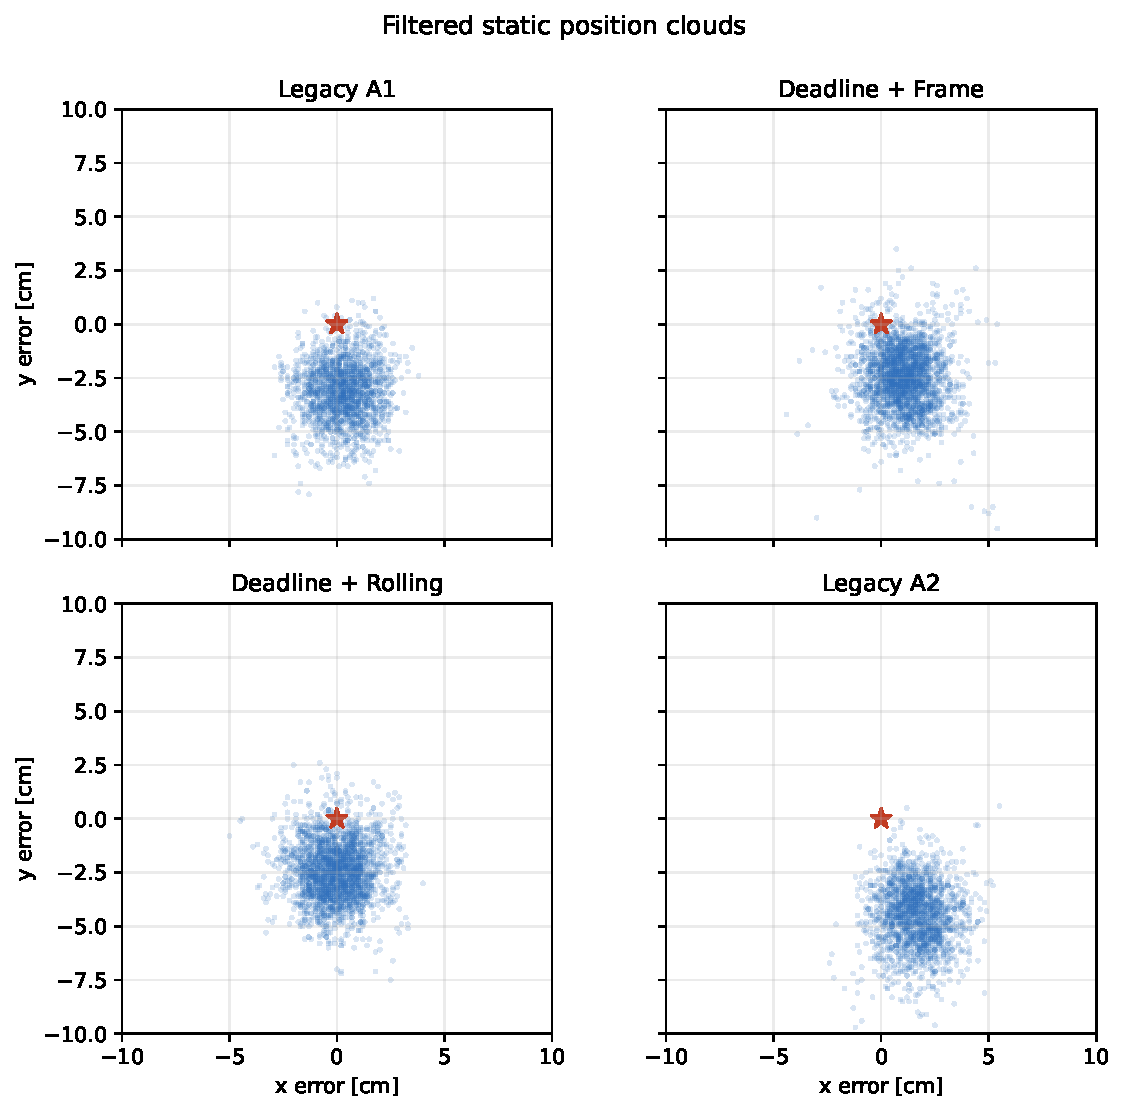
\includegraphics[width=0.90\linewidth]{pipeline_position_clouds.pdf}
\caption{Filtered position clouds relative to the surveyed centre.}
\end{figure}

\FloatBarrier
\subsection{Confidence-band acceptance}

A moving-block bootstrap with 3,000 iterations was used to retain temporal
correlation. The acceptance rule requires both the candidate point RMSE and
P95 to remain no greater than the upper 95\% confidence bound of the
same-geometry control.

\begin{table}[htbp]
\centering
\small
\begin{tabular}{lrrrrl}
\toprule
Comparison & metric & control & control upper & candidate & result\\
 & & [cm] & 95\% bound [cm] & [cm] &\\
\midrule
Deadline Frame vs Legacy A1 & RMSE & 3.59 & 3.71 & 3.23 & accepted\\
 & P95 & 5.51 & 5.76 & 5.09 & accepted\\
Rolling frames vs Deadline Frame & RMSE & 3.23 & 3.36 & 3.01 & accepted\\
 & P95 & 5.09 & 5.30 & 4.72 & accepted\\
\bottomrule
\end{tabular}
\caption{Predefined accuracy gates.}
\end{table}

Both candidate configurations pass. These data demonstrate no observed
accuracy regression; they do not yet prove that deadline scheduling improves
accuracy in all conditions. The captures were sequential and the live geometry
estimator continued to evolve.

\section{Radio-pipeline diagnostics}

\begin{table}[htbp]
\centering
\small
\begin{tabular}{lrrrrrrr}
\toprule
Mode & complete & RESP TO & FINAL TO & collision & overrun &
invalid & re-arm fail\\
\midrule
Legacy + Frame A1 & 23,791 & 1,914 & 619 & 0 & 0 & 0 & 0\\
Deadline + Frame & 32,128 & 408 & 277 & 672 & 39 & 0 & 0\\
Deadline + Rolling & 32,585 & 305 & 275 & 620 & 41 & 0 & 0\\
\bottomrule
\end{tabular}
\caption{Counters accumulated across all modules during each 60 s interval.
TO denotes timeout.}
\end{table}

\begin{figure}[htbp]
\centering
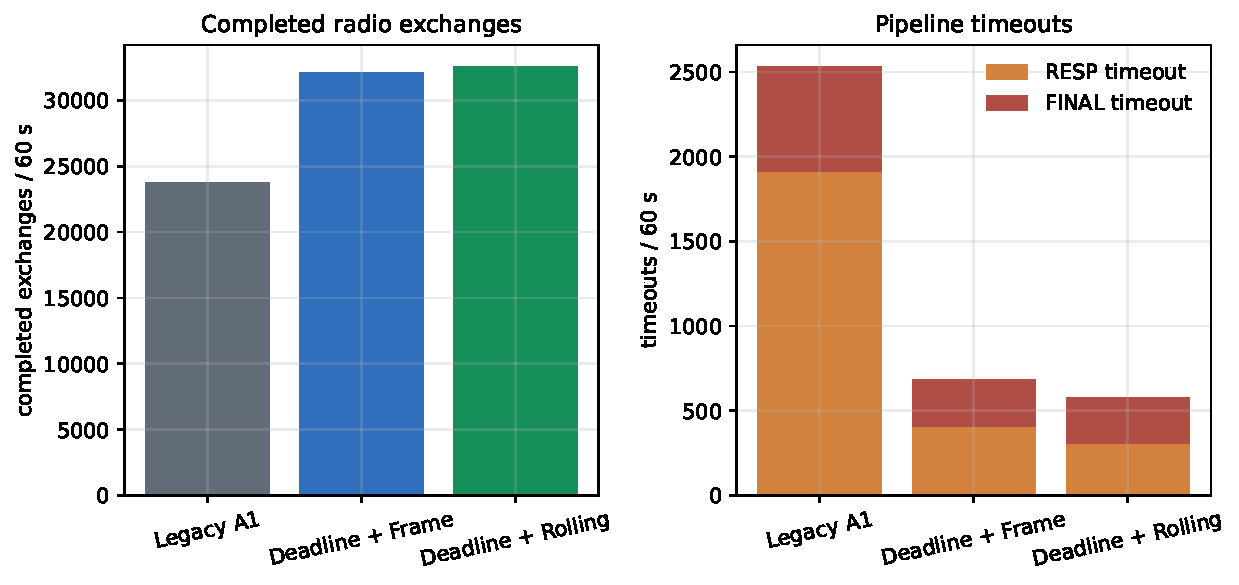
\includegraphics[width=0.96\linewidth]{pipeline_diagnostics.pdf}
\caption{Completed exchanges and timeout counts.}
\end{figure}

Compared with Legacy A1, Deadline + Frame completed approximately 35\% more
exchanges and reduced combined RESP/FINAL timeout counts from 2,533 to 685,
a reduction of approximately 73\%. No invalid frame or RX re-arm failure was
reported. CIA readout averaged approximately 25--42 \(\mu\)s across modules,
while RX re-arm averaged 38--46 \(\mu\)s.

The deadline schedule exposes state collisions and rare schedule overruns that
were not explicit counters in the Legacy path. They remain useful optimisation
targets, but did not prevent the measured throughput gain. Timer alarm counts
are normal deadline wake-ups and are not failure events.

\FloatBarrier
\section{Anchor-geometry stability}

\begin{figure}[htbp]
\centering
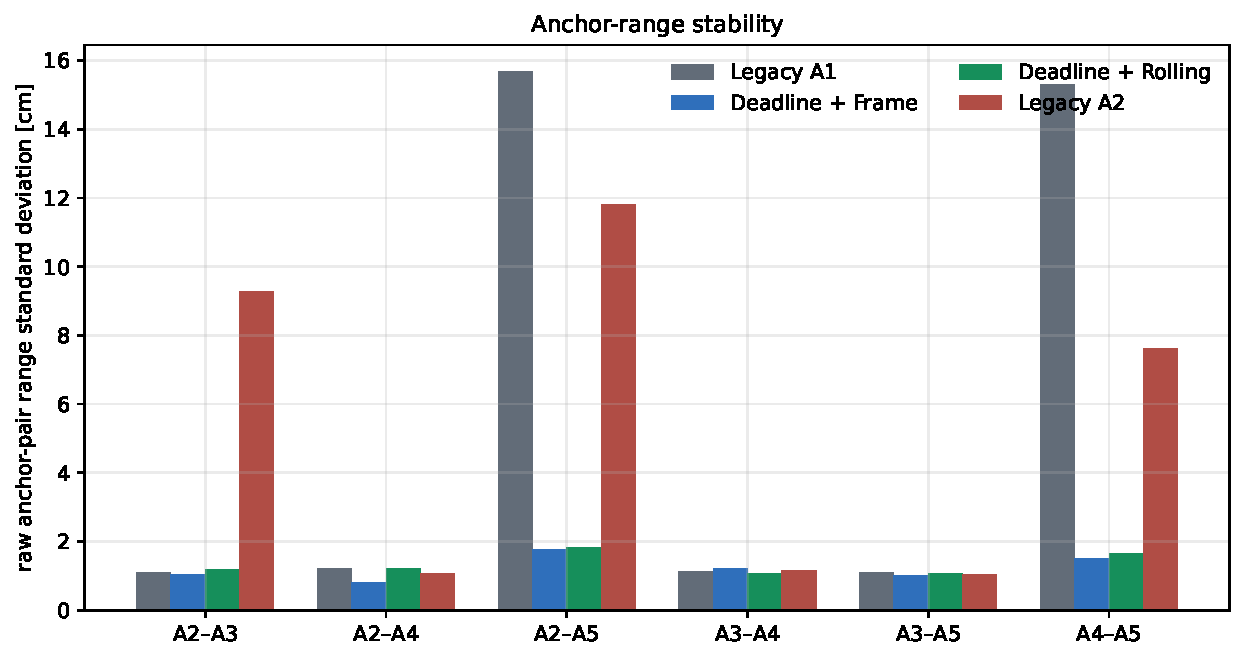
\includegraphics[width=0.84\linewidth]{pipeline_anchor_stability.pdf}
\caption{Standard deviation of raw anchor-pair DS-TWR ranges.}
\end{figure}

Deadline + Frame kept every anchor-pair standard deviation at or below
1.78 cm. Both Legacy captures contained intermittent bursts. In A2, standard
deviation reached 9.27 cm on A2--A3, 11.81 cm on A2--A5, and 7.62 cm on
A4--A5. These bursts explain the degraded A2 position cloud and match the
short-lived geometry deformations previously observed in the dashboard.

Mean anchor-pair biases of several centimetres remain. They are a separate
antenna/pair-calibration issue and should not be attributed to deadline
scheduling. The present experiment evaluates relative scheduling behaviour,
not a new absolute calibration.

\FloatBarrier
\section{Conclusions}

\begin{enumerate}[itemsep=2pt,topsep=3pt]
\item The DW3000 deadline pipeline reaches approximately
\textbf{84 independent positions/s}, essentially the previously observed
FlexTDOA target rate, while keeping the native 1.0/1.0 ms radio timing.
\item Both filtered and raw accuracy gates pass. No accuracy concession was
required to obtain the throughput gain.
\item Rolling solving delivers approximately \textbf{169 display updates/s}
without reducing independent frame throughput. Its additional results are
correlated and must continue to be reported separately.
\item Deadline scheduling materially reduces timeout counts and anchor-range
bursts. This should also improve the stability of live anchor self-localisation.
\item Remaining work should focus on the recorded state collisions, rare
schedule overruns, and static pair/antenna bias calibration. A longer
randomised or interleaved field campaign is required before claiming a general
accuracy improvement.
\end{enumerate}

\medskip
\noindent\textbf{Operational state and reproducibility.}
All modules were left online in Deadline + Rolling at 100 Hz with Robust
Rotating 1.0/1.0 ms; the dashboard remained active. The report directory
contains all captures, metadata, timing logs, bootstrap outputs, metrics, and
the reproducible report generator in \texttt{tools/}.

\end{document}
